  \ac{RIA} ist kein Standard, sondern ein synonym für Applikationen, welche
  eine ``reichhaltige'' Benutzeroberfläche bieten und eine Verbindung mit dem
  Internet haben. Siehe \cite{RichInternetApplication} und
  \cite{RichInternetApplicationsWhitePaper} S. 2.
  
  \section{Grundlagen}
  
  Der Begriff \ac{RIA} ist mit der Entwicklung des Internets entstanden und
  wird heute oft verwendet. Für viele Leute ist \ac{RIA} ein synonmy für
  Webanwendungen, welche mit \ac{Ajax} realisiert werden. \ac{Ajax} bietet die
  Möglichkeit eine ``reichhaltige'' Benutzeroberfläche zu entwickeln, so wie
  man sich das von klassischen Desktopanwendungen gewöhnt ist. Die Grenze
  zwischen der klassischen Webanwendung und einer Desktopapplikation scheint
  damit zu verschwinden. Genauer betrachtet steht eine \ac{RIA} im
  Technologiespektrum aber zwischen dem Rich Client und dem Thin Client, siehe
  Abbildung \ref{img:webanwendungen}.
  
  \begin{figure}[h]
    \begin{center}
      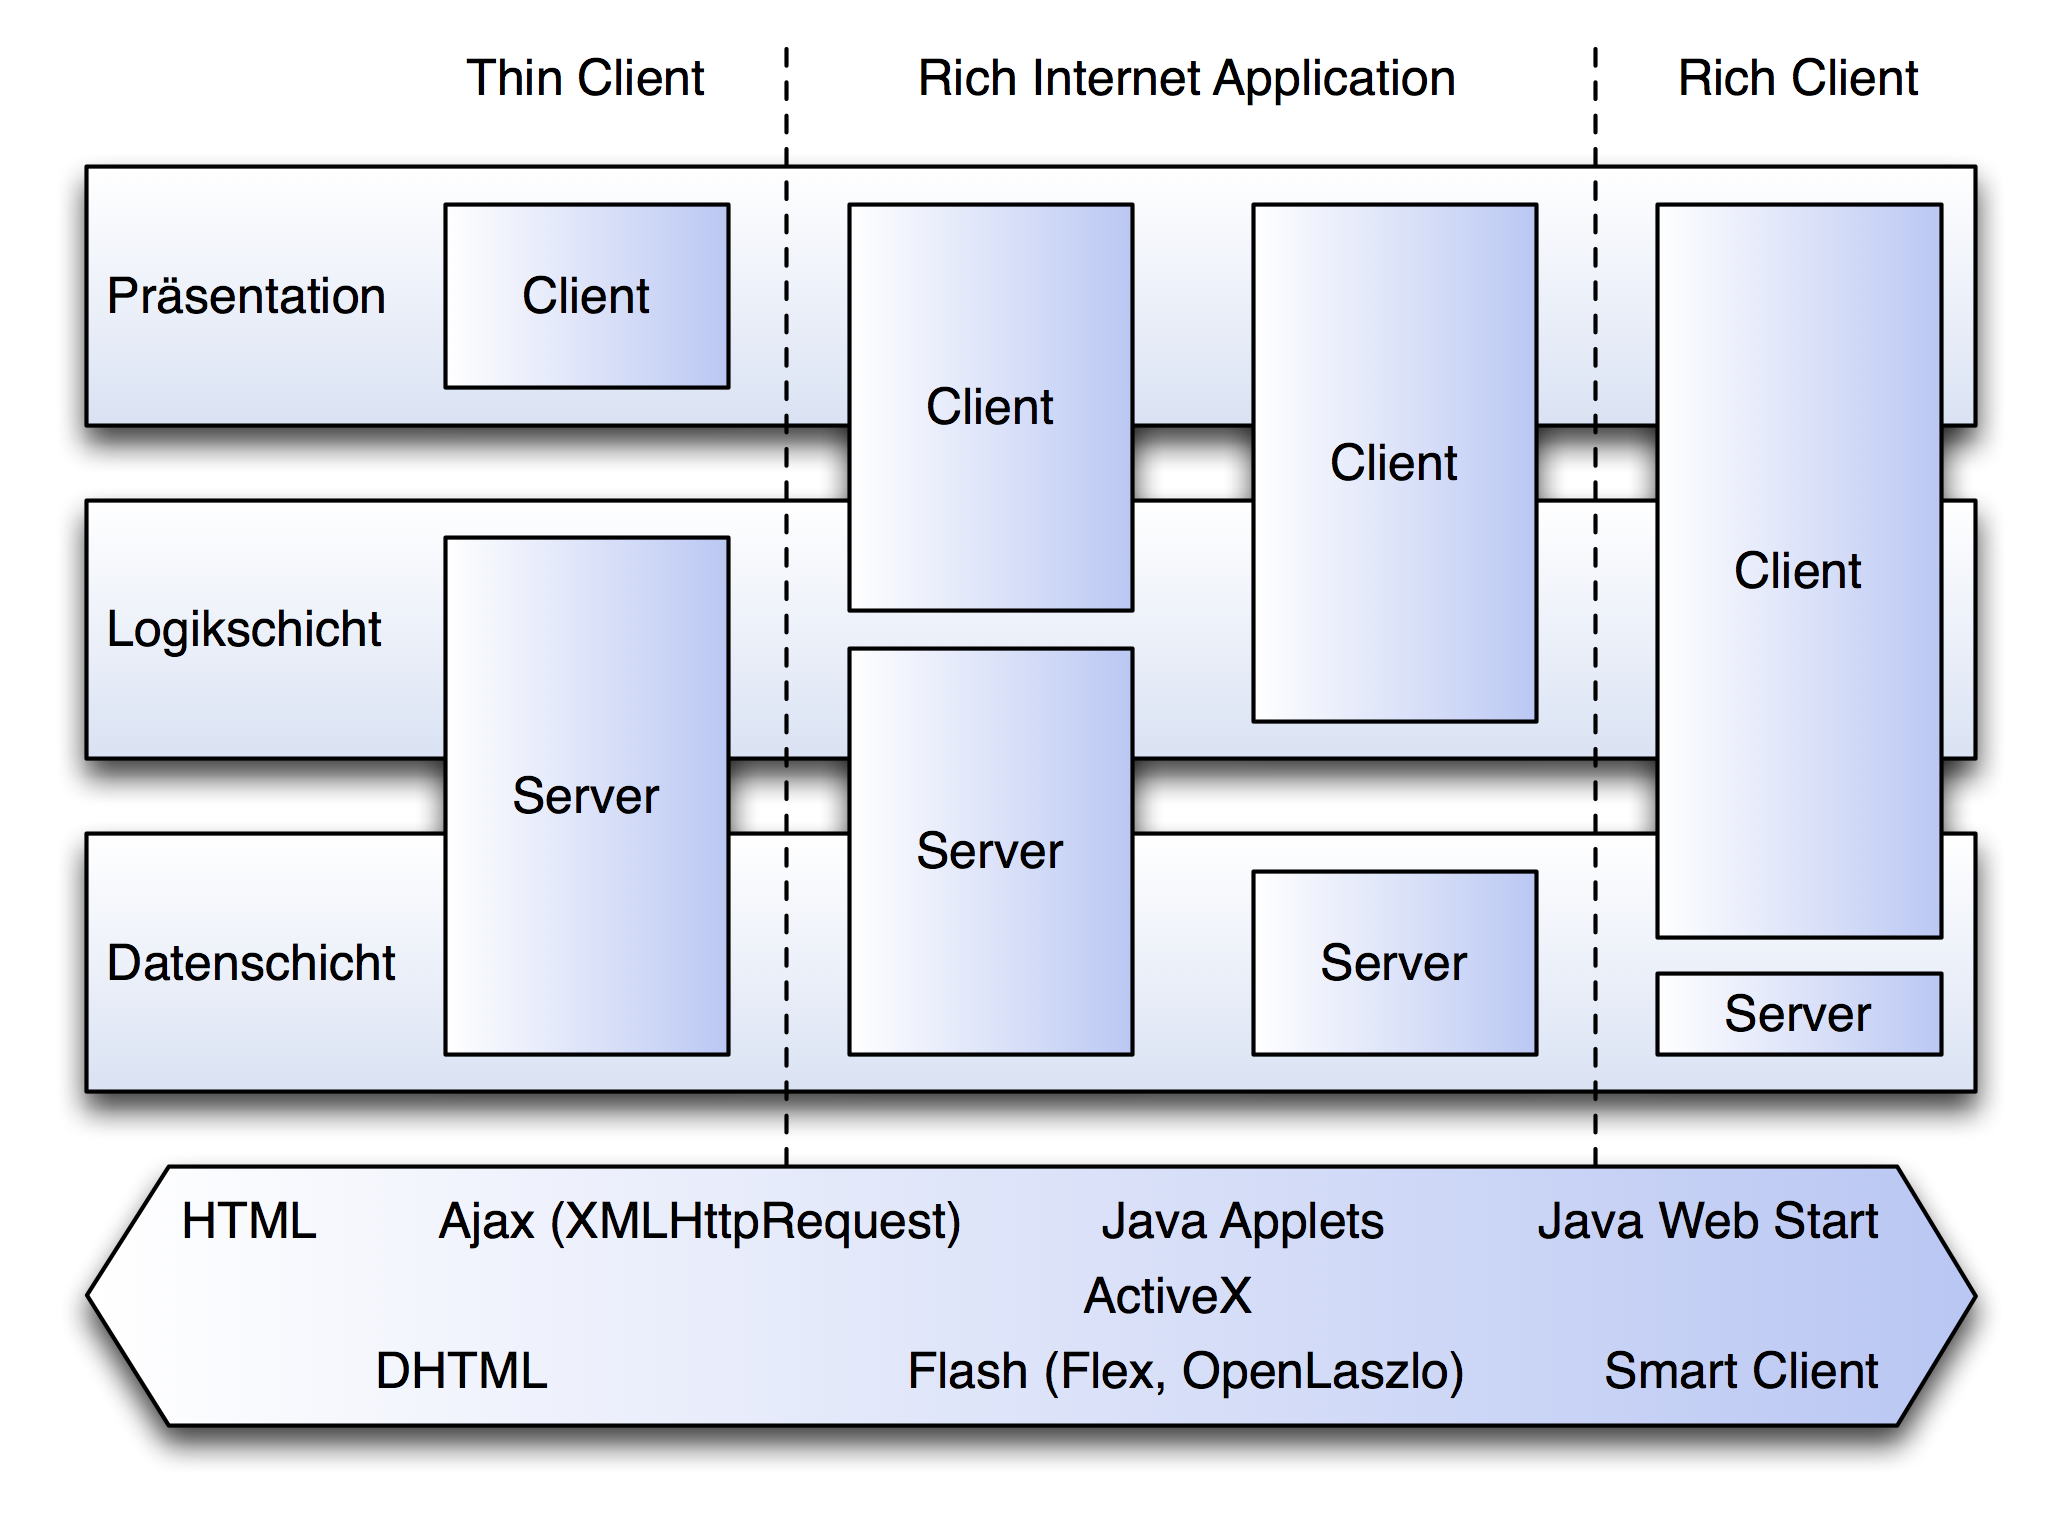
\includegraphics[width=0.7\textwidth]{./image/webanwendungen.png}
      \caption{Web Anwendungen (nach \cite{DiplomarbeitStephanSchuster} S. 6f.
      und \cite{WebApplicationSolutions} S. 5)}
      \label{img:webanwendungen}
    \end{center}
  \end{figure}
  
  Rich Client steht für kompilierte Desktopapplikationen und Thin Client für
  Webapplikationen welche im Webbrowser laufen, siehe
  \cite{WebApplicationSolutions} S. 4f. Da die Grenze zwischen \ac{RIA} und
  Thin Client nicht klar definiert ist, werden diese beiden Begriffe zum Teil
  als Synonym verwendet.
  
  \section{Klassifikation}
  
  Es wird eine Klassifikation aller \ac{RIA} in die Klassen der Plugin
  orientierten, der Client orientierten und der Browser orientierten gemacht.
  
  \subsection{Plugin orientiert}
  
  Plugin orientierte \ac{RIA} sind Applikationen, welche in einem Browser
  Plugin laufen. Dabei sind Adobe Flash, Java Applet und Microsoft Silverlight
  die drei grössten Vertreter in dieser Sparte, siehe \cite{RichInternetApplications}
  und \cite{RichInternetApplicationMarketShare}.

  \subsection{Client orientiert}
  
  Unter Client orientiert versteht man lediglich, dass alle Desktopanwendungen,
  welche entweder mit den Internet kommunizieren oder zumindes über dieses
  ausgeliefert werden, zu dieser Kategorie gehören. Dies trifft nur zu, in der
  Annahme, dass Desktopanwendungen eine ``reichhaltige'' Bedienoberfläche
  anbieten, siehe \cite{RichInternetApplication}. Eine Java Swing Applikation
  könnte also auch als Client orientierte \ac{RIA} klassifiziert werden.
  
  \subsection{Browser orientiert}
  
  Browser orientierte \ac{RIA} kommen aus der Evolution der Internettechnologie
  heraus. Da sich die Grundkonzepte der Internettechnologie in den letzten
  Jahren stark verändert haben, müssen wir zwischen klassischen Webanwendungen
  und Webanwendungen mit Ajax unterscheiden.
  
  \subsubsection{Klassische Webanwendung}
  
  Um die Jahrtausenwende wurden klassische Webanwendung nach dem Prinzip von
  Request - Response aufgebaut. Der Benutzer konnte mit einer Interaktion einen
  Statuswechsel von einer Seite zur Nächsten auslösen, zum Beispiel durch das
  anklicken eines Links oder mit dem Versenden eines HTML-Formulars, siehe
  Abbildung \ref{img:classicPageReload}. Der zeitliche Ablauf sieht mit einem
  \ac{UML} Sequenzdiagramm wie folgt aus, siehe Abbildung
  \ref{img:sequenzdiagrammClassicPageReload}. Dabei wurde immer der gesamte
  Seiteninhalt neu geladen, was zu langen wartezeiten beim Laden der Seite und
  zu einem ungewohnten Anwendergefühl, im Vergleich zu Desktopanwengungen,
  geführt hat. Zudem wurden immer alle Daten vom Server an den Browser
  übermittelt, welche für die Darstellung der Webanwendung von Nöten war, siehe
  \cite{AjaxInAction} S. 44ff.
  
  \begin{figure}[hbt]
    \begin{center}
      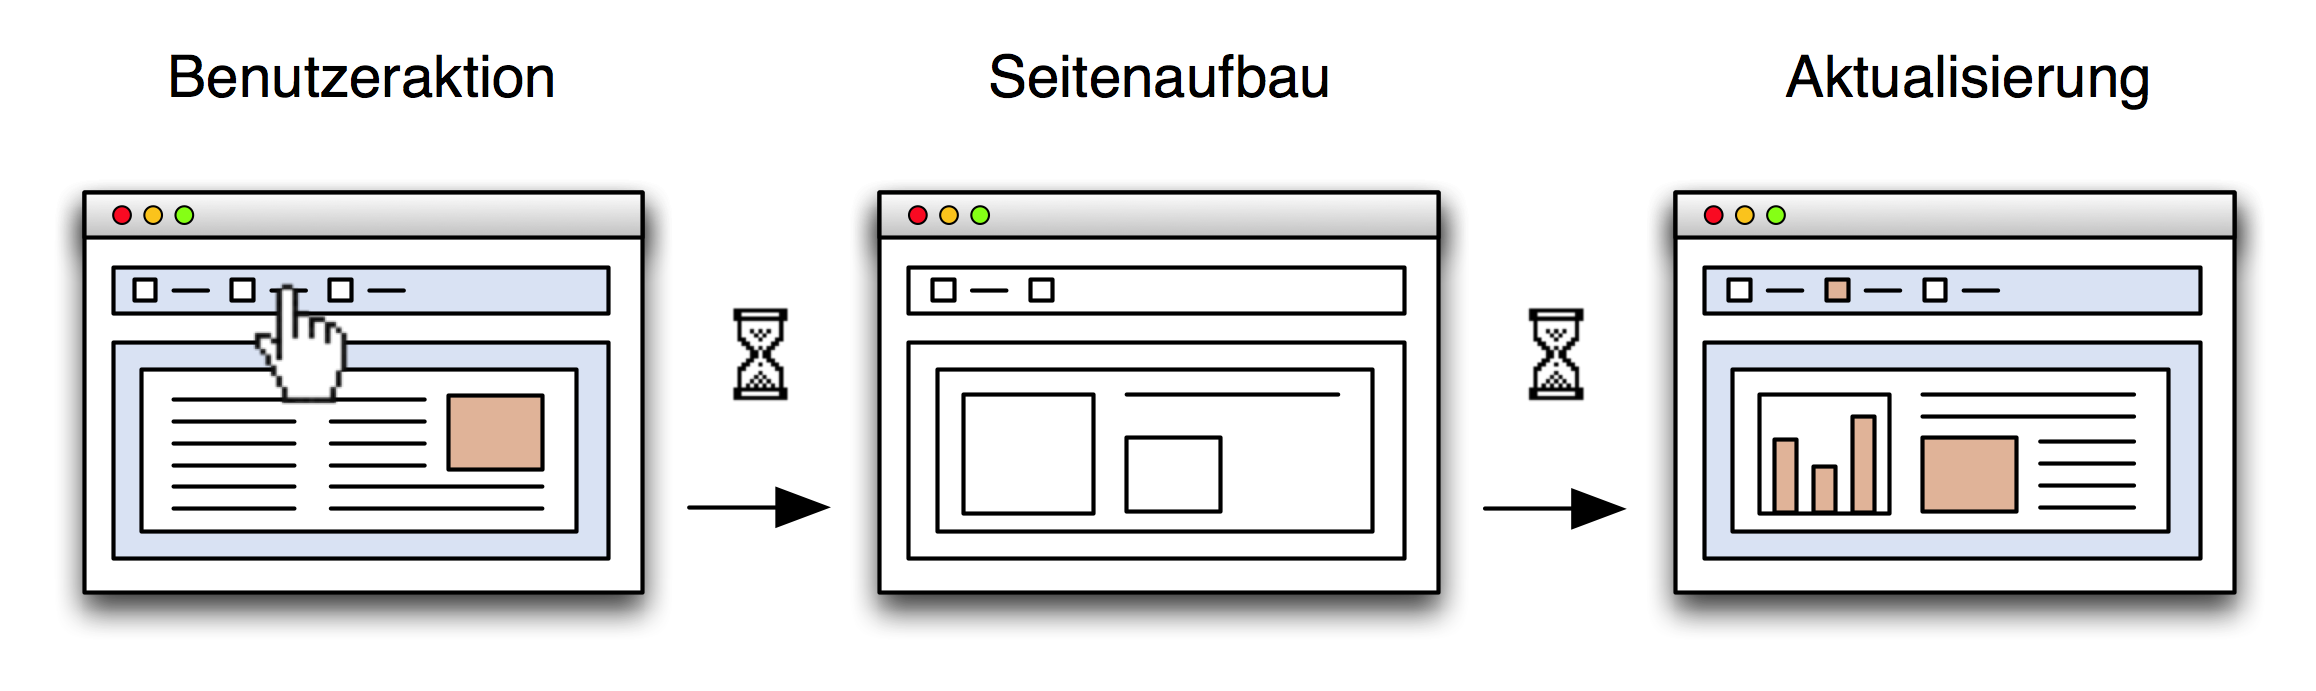
\includegraphics[width=\textwidth]{./image/classicPageReload.png}
      \caption{Klassische Webanwendung aus der Usersicht (nach
      \cite{DiplomarbeitStephanSchuster} S. 10)}
      \label{img:classicPageReload}
    \end{center}
  \end{figure}
  
  \begin{figure}[hbt]
    \begin{center}
      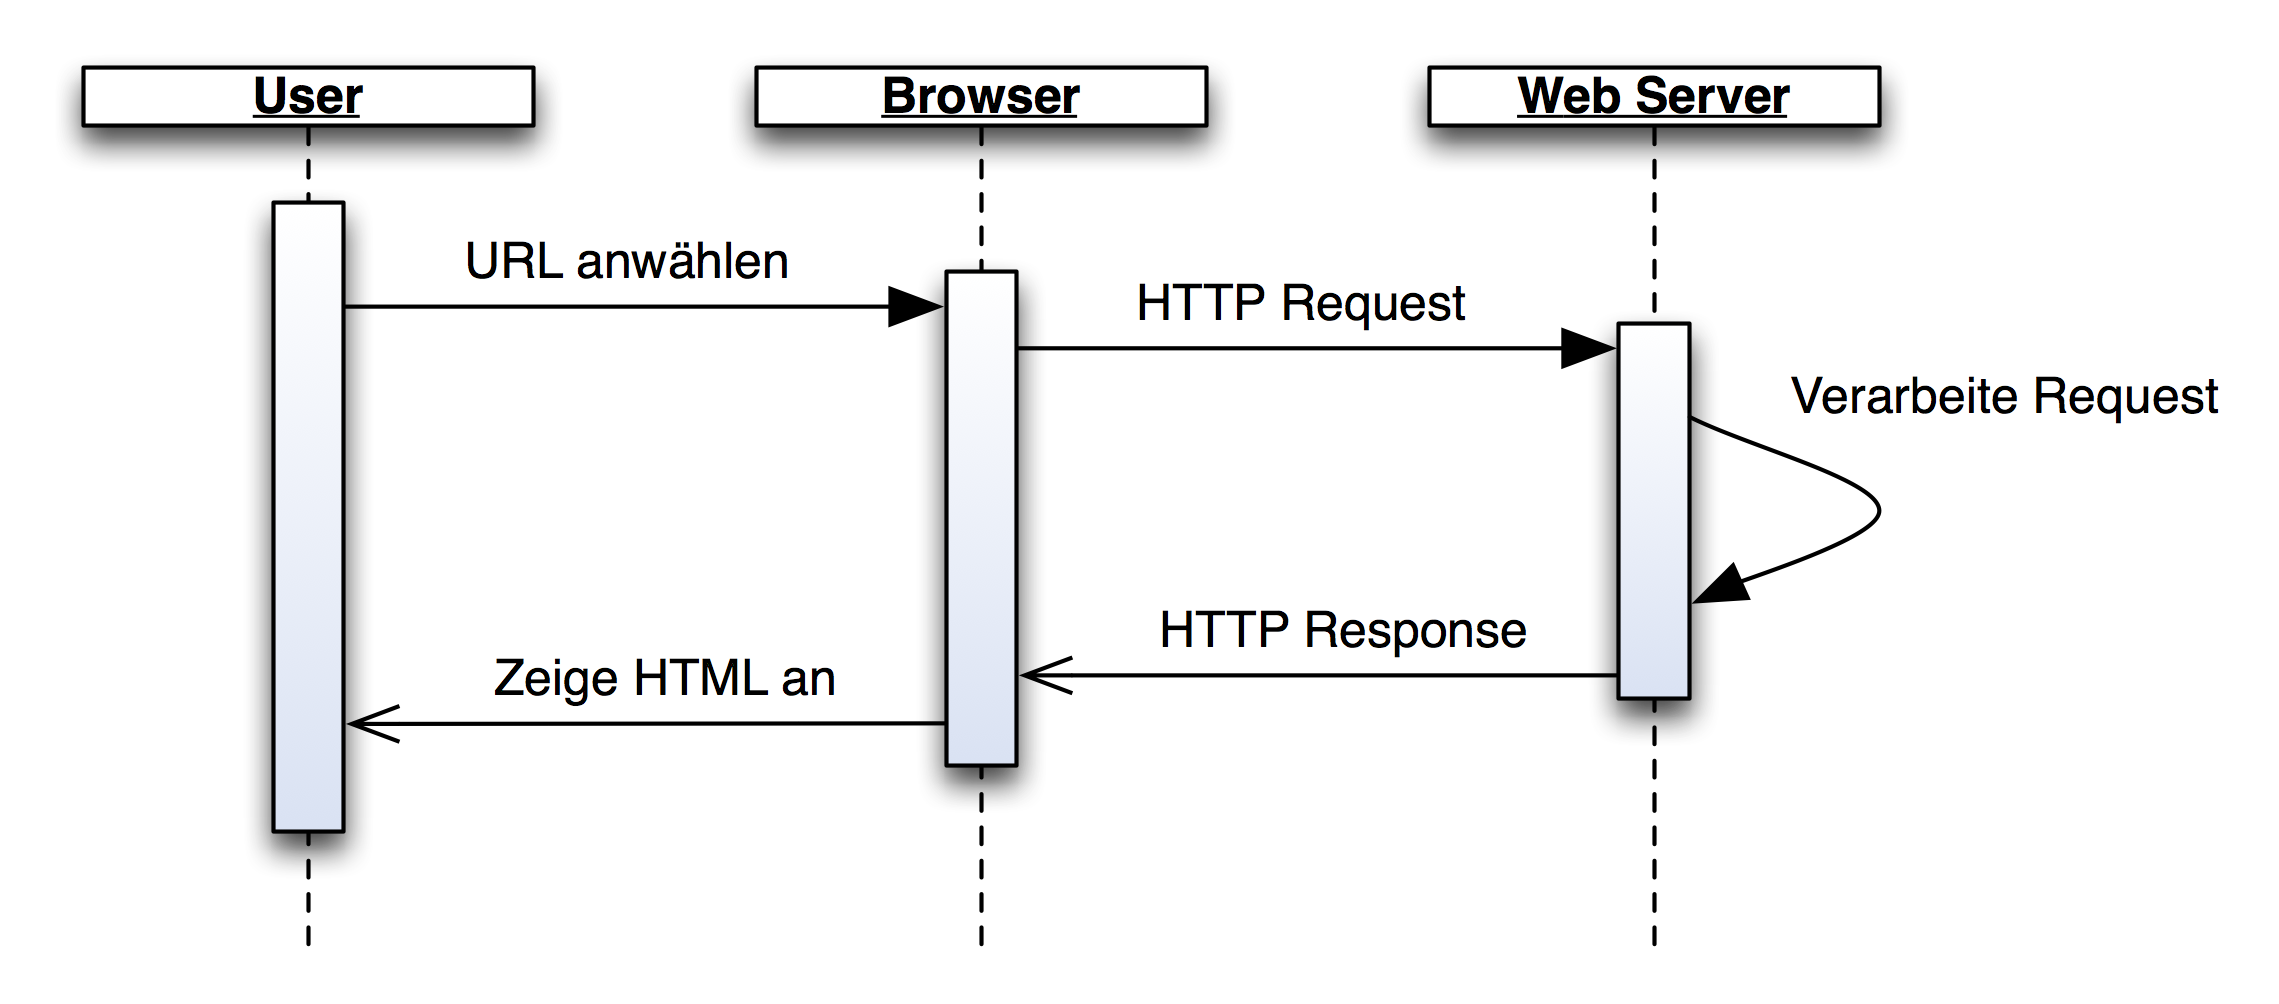
\includegraphics[width=\textwidth]{./image/sequenzdiagrammClassicPageReload.png}
      \caption{HTTP Request als \ac{UML} Sequenzdiagramm (nach
      \cite{HttpBasics} S. 10)}
      \label{img:sequenzdiagrammClassicPageReload}
    \end{center}
  \end{figure}
  
  \subsubsection{Webanwendung mit Ajax}
  
  Mit dem Konzept von \ac{Ajax}, bei dem der Browser asynchron Daten vom Server
  nachladen kann, wurde die Möglichkeit geschaffen, Anwendungen zu entwickeln,
  welche sich in der Bedienung wie Desktopanwendungen anfühlen, siehe Abbildung
  \ref{img:ajaxPageReload}. Der zeitliche Ablauf sieht mit einem \ac{UML}
  Sequenzdiagramm wie folgt aus, siehe Abbildung
  \ref{img:sequenzdiagrammAjaxPageReload}. Das Prinzip funktioniert dadurch,
  dass eine zusätzliche Schicht zwischen dem Browser und Server eingerichtet
  wird. Diese Schicht, ich nenne sie hier Ajax-Engine, übernimmt die Kontrolle
  über die Datenkommunikation zum Server. Die Ajax-Engine bietet die
  Möglichkeit asynchron zur Clientinteraktion Daten vom Server anzufordern und
  bei Erhalt dynamisch in die bestehende Seite einzuflechten. Das Ergebnis ist,
  dass der Browser vom Server entkoppelt wird, wobei der Benutzer die Seite
  weiterhin verwenden kann. Der Server kann nun im Hintergrund getätigte
  Interaktionen verarbeiten.
  
  \begin{figure}[hbt]
    \begin{center}
      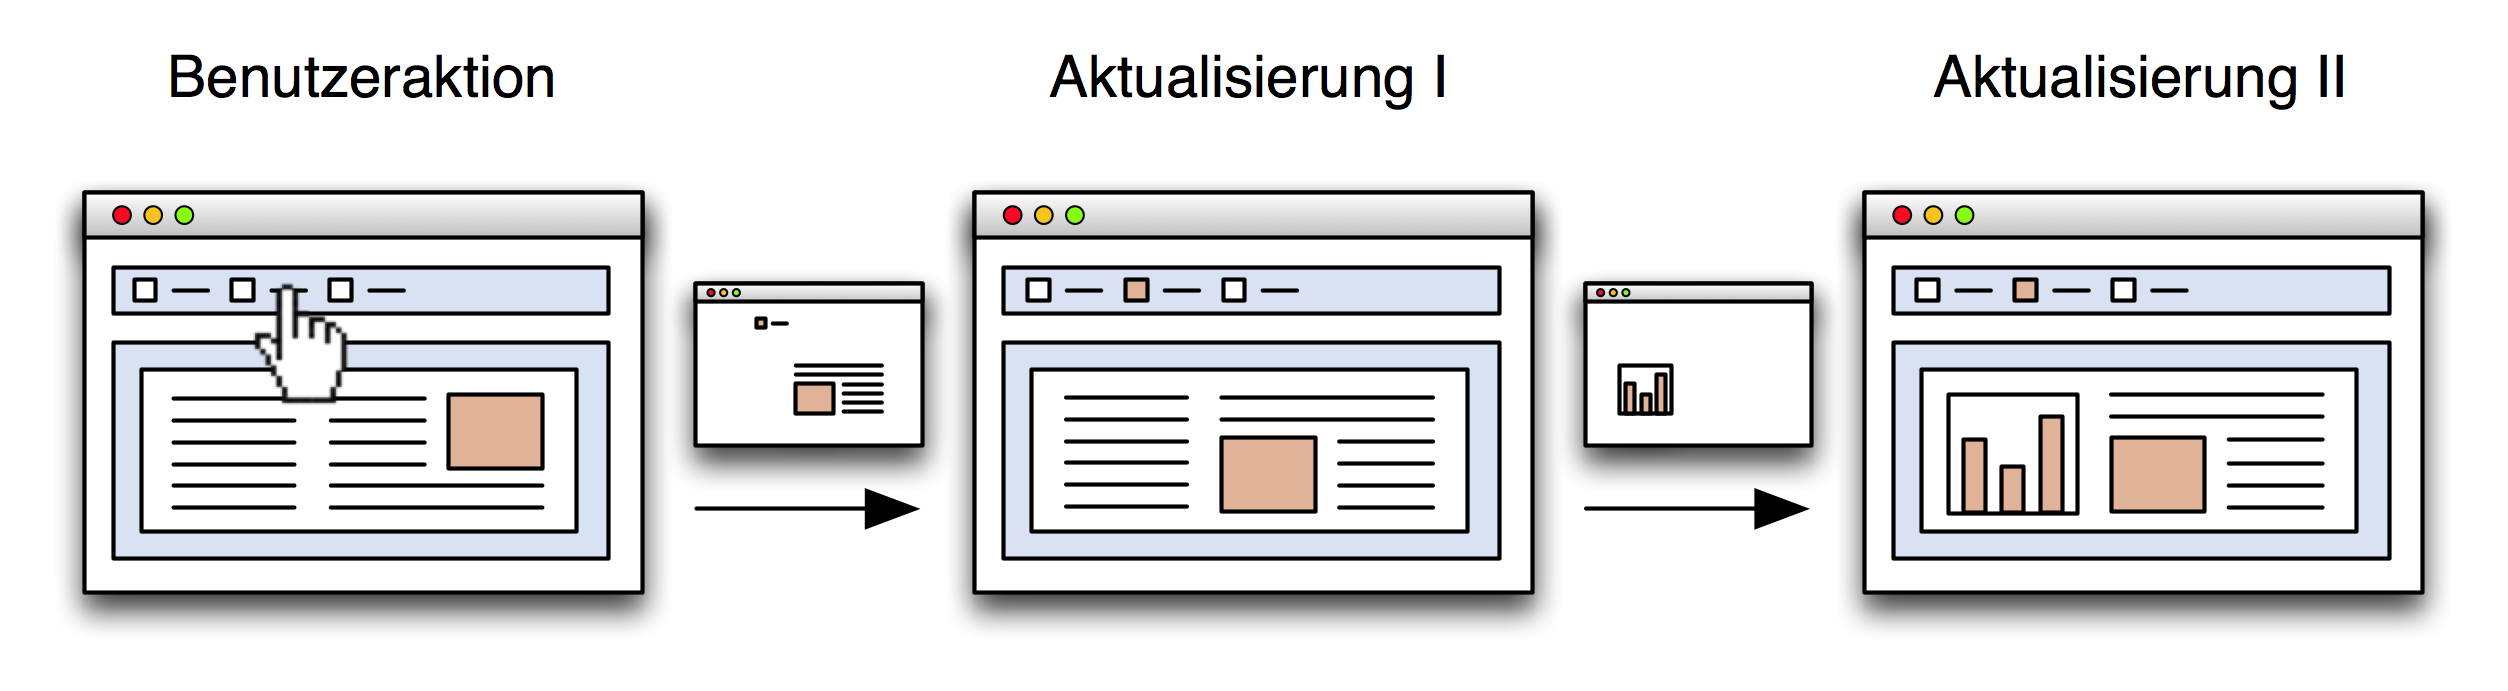
\includegraphics[width=\textwidth]{./image/ajaxPageReload.png}
      \caption{Webanwendung mit Ajax aus der Usersicht (nach
      \cite{DiplomarbeitStephanSchuster} S.12)}
      \label{img:ajaxPageReload}
    \end{center}
  \end{figure}
  
  \begin{figure}[hbt]
    \begin{center}
      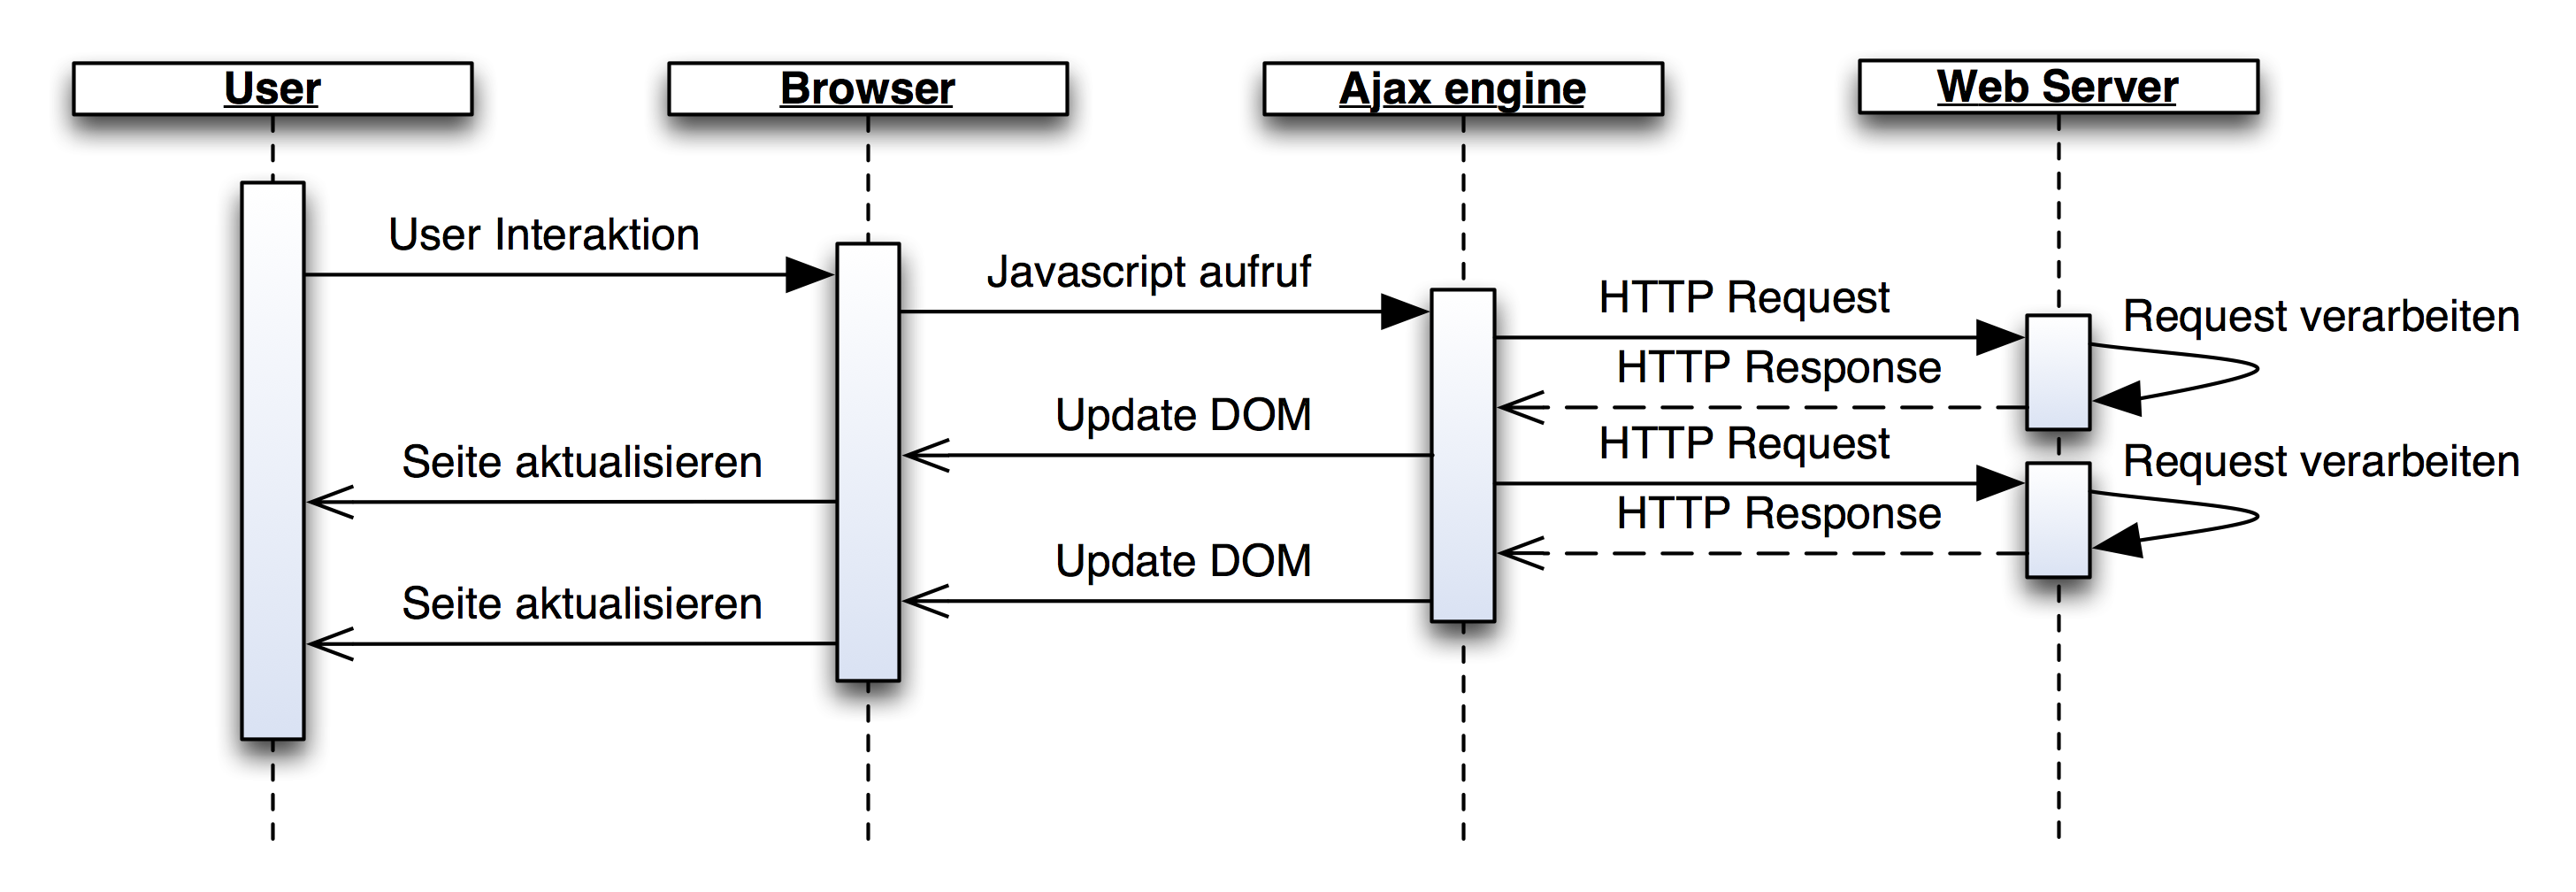
\includegraphics[width=\textwidth]{./image/sequenzdiagrammAjaxPageReload.png}
      \caption{Ajax Request als \ac{UML} Sequenzdiagramm}
      \label{img:sequenzdiagrammAjaxPageReload}
    \end{center}
  \end{figure}
  
  \subsubsection{Security}
  
  Nach \cite{RichInternetApplication} gelten Browser orientierte \ac{RIA},
  welche auf Webstandards\footnote{Webstandards werden durch das Gremium W3C
  definiert, siehe \url{http://www.w3.org/}} basieren, als relativ sicher.
  Mögliche Sicherheitslöcher stellen vorallem der jeweils verwendete Browser,
  in der die Applikation dargestellt wird, und Attacken nach dem Prizip von
  Social Engineering\footnote{Bei Social Engineering geht es darum, durch
  zwischenmenschliche Beeinflussung, unberechtigt an Daten oder Dinge zu
  gelangen, siehe \cite{SocialEngineering}}.
  
  \subsubsection{Suchmaschinenoptimierung}
  
  Suchmaschinenoptimierung dient dazu im Ranking einer Suchmaschine besser
  abzuschliessen. Dies ist vorallem bei Unternehmen von Bedeutung, welche das
  Internet als Vertriebkanal sehen. Bei statischen Webseiten ist das Indexieren
  ein Prozess der gut funktioniert. Bei einer \ac{RIA}, welche über \ac{Ajax}
  Daten zur Laufzeit einer Webapplikation asynchron nachlädt, wird das für eine
  Suchmaschine ein schwierigeres Unterfangen, die Daten Sinnvoll abzugreifen.
  
  \section{Vorgaben aus der IT-Architektur der Zürcher Kantonalbank}
  
  In der Zürcher Kantonalbank gibt es klare Vorschriften, welche Arten von
  \ac{RIA} eingesetzt werden dürfen. Diese Vorschriften werden im Handbuch der
  IT-Architektur zusammengefasst, siehe \cite{ZkbHandbuchDerItArchitektur} S.
  140ff. 
  
  \subsection{Restriktion}
  
  Aus den Vorschriften der IT-Architektur, geht hervor, dass keine neuen
  Applikationen als Plugin orientierte \acp{RIA} entwickelt werden, siehe
  \cite{ZkbHandbuchDerItArchitektur} S. 143f. Zudem wird festgelegt, dass
  Client orientierte \acp{RIA} für neue Applikationen nicht in Frage kommen,
  falls die Business-Logik im Client liegt, siehe
  \cite{ZkbHandbuchDerItArchitektur} S. 141f.
  
  \subsection{Mögliche Implementierung}
  
  Als mögliche Implementierung werden von der IT-Architektur der \ac{ZKB} zwei
  Gruppen genannt. Die Gruppe der Thin Clients und die Gruppe der Ultra Thin
  Clients. Die Gruppe der Thin Clients ist gemäss dem IT-Architektur Handbuch
  eine Java Desktop Applikation, welche nur eine Präsentations-Logik enthält.
  Die Gruppe der Ultra Thin Clients entspricht den Browser orientierten
  \ac{RIA}, siehe Abbildung \ref{img:zkbWebAnwendungen}
  
  \begin{figure}[hbt]
    \begin{center}
      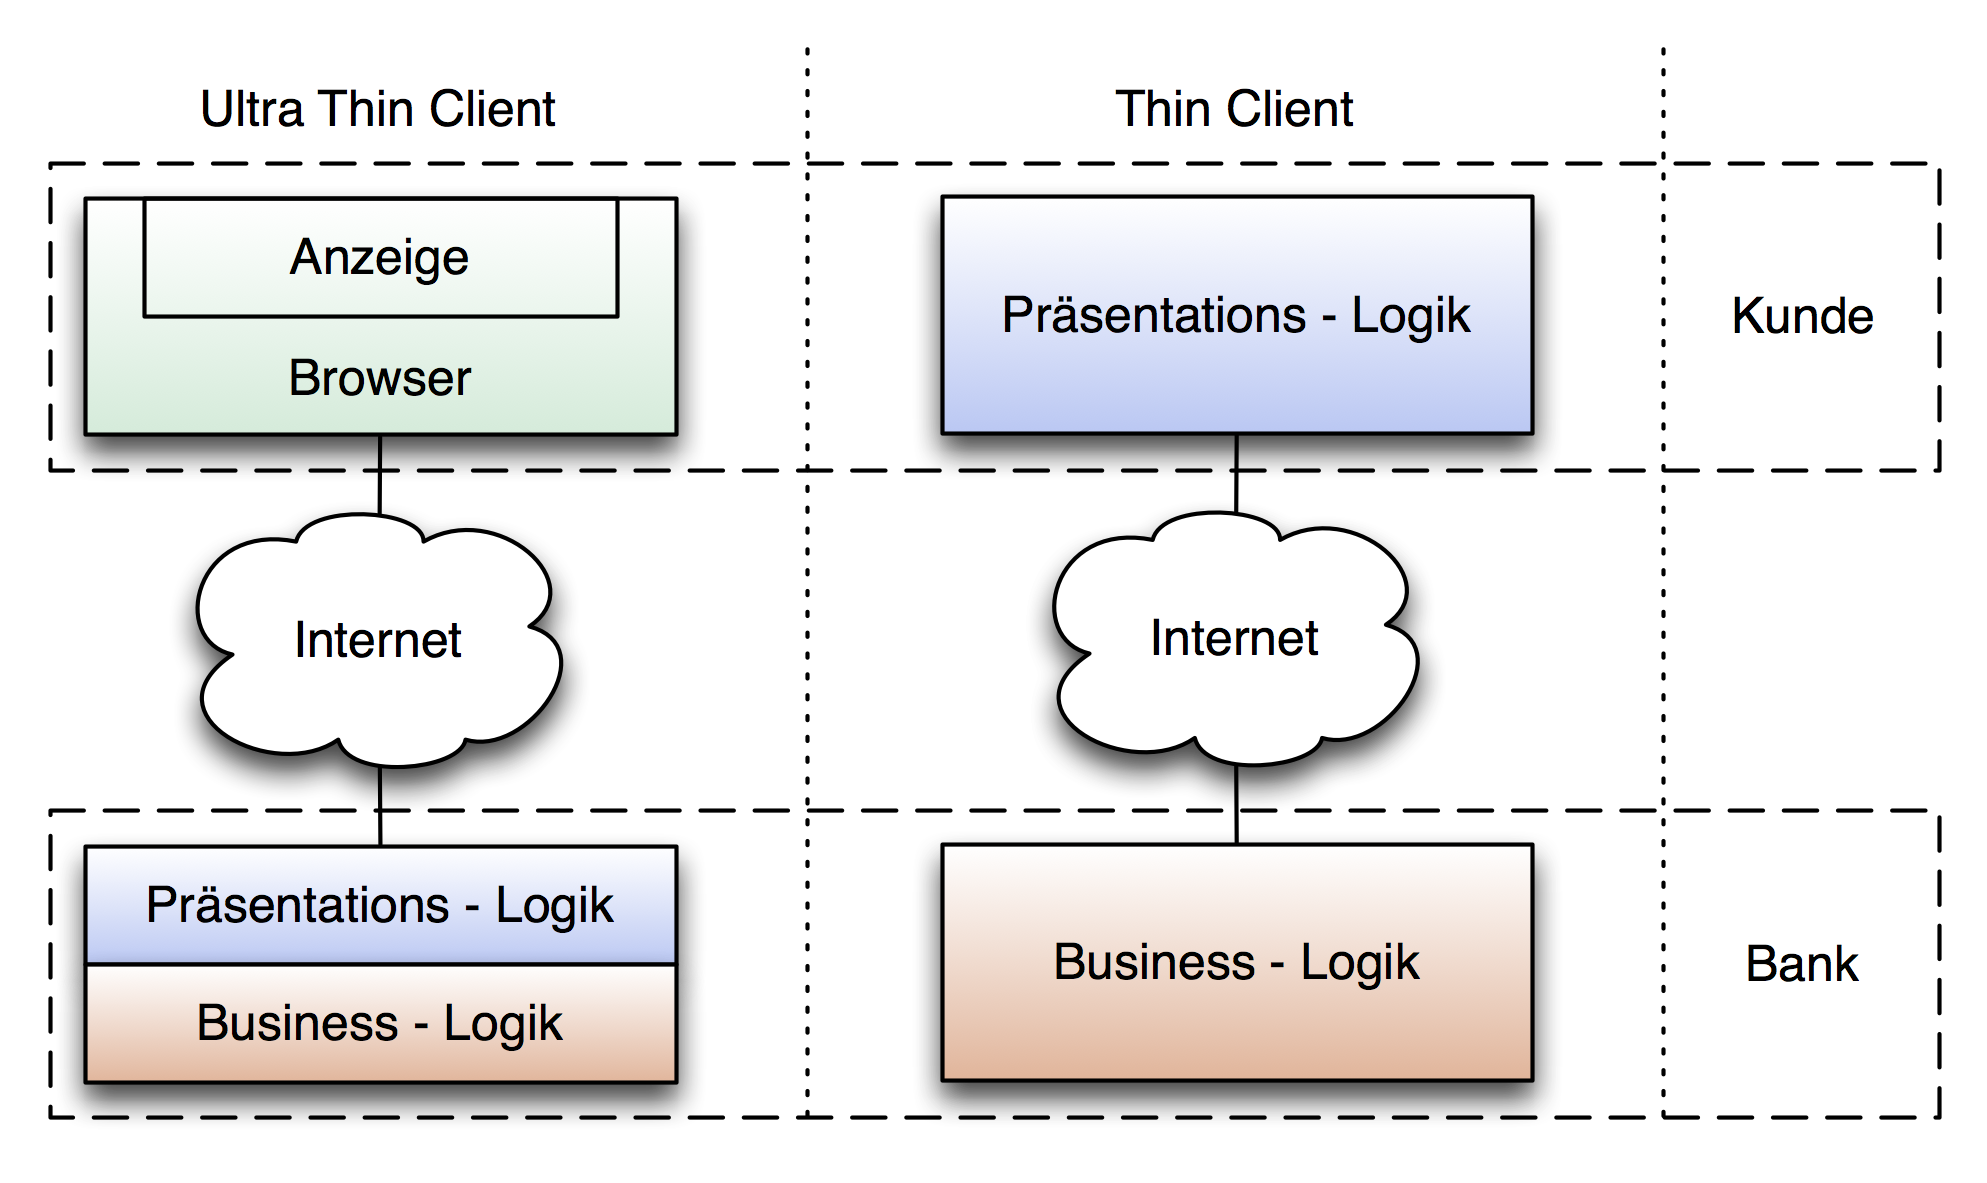
\includegraphics[width=\textwidth]{./image/zkbWebAnwendungen.png}
      \caption{Möglicher Aufbau von Web Applikationen (nach
      \cite{ZkbHandbuchDerItArchitektur} S. 141)}
      \label{img:zkbWebAnwendungen}
    \end{center}
  \end{figure}
  